\subsection{Mechanic\label{Mechanic}}

%\begin{figure*}[htb]
\begin{center}
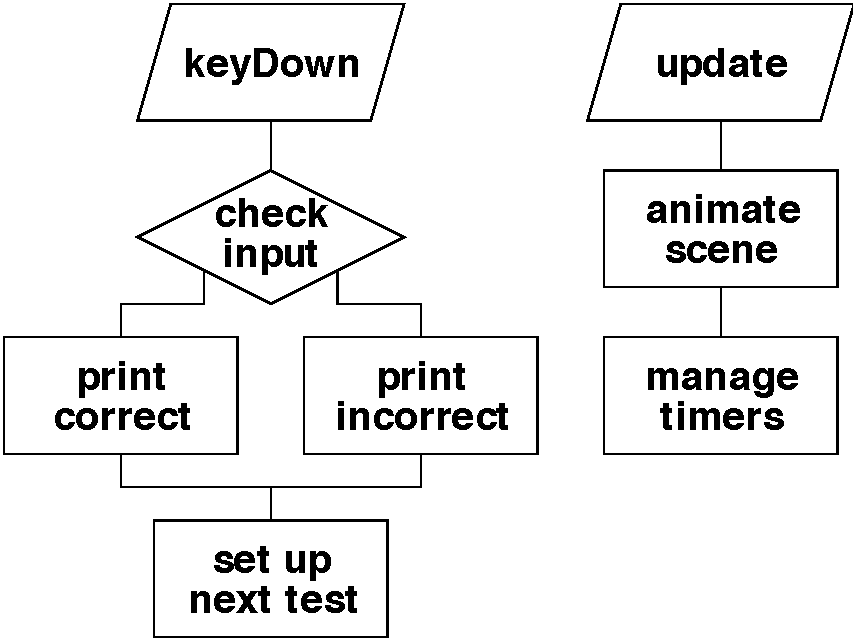
\includegraphics[width=7cm]{media/code.pdf}
%\caption{A diagram of a possible scene graph.\label{imgCode}}
\end{center}
%\end{figure*}

\paragraph{}
In the current version, scene mechanic is closely tied to Lua.
The interaction of the scene with the subject as well as internal actions such as animation are defined in \textit{lua} script, and executed by the \textit{lua} engine.

By modifying the class \lstinline{Program} it would be possible to replace lua with a custom interpreter for an other language.
A graphical programming launguage or a key-frame interpolation class are possible replacements.

\subsubsection{Event Model}
\paragraph{}
Lua does not have a run loop or a main function.
It consists of code that is executed on load and functions that are called from \ER.
Once a scene has done the desired actions it is expected to return control to the program.

To easily integrate into \ER's model, event handler functions can be registered to receive notifications and execution control.
Three event handlers are commonly used: \lstinline{keyDown}, \lstinline{keyUp} and \lstinline{update}.
\lstinline{keyDown} is called when ever a key is pressed.
\lstinline{keyUp} is called when the key is released again.
\lstinline{update} is called in regular intervals, currently roughly thirty times per second.

\subsubsection{Binding}
The class \lstinline{LuaProxy} encapsulates the \textit{lua} engine.
It contains glue code to bind functionality from \textit{lua} to \textit{C++} and manages the event handlers.
Objects (see \ref{ImplObject}) are bound to lua with the \textit{LuaBridge} library.
This library handles almost all of the bridging, only in special cases, like enum parameters, objects have to provide custom methods.

